\documentclass[CMPE]{KGCOEReport}
\usepackage{float}
\usepackage{adjustbox}
\graphicspath{ {./images/} }

\newcommand{\name}{Mohammed Fareed \\ Trent Wesley}
\newcommand{\exerciseNumber}{8}
\newcommand{\exerciseDescription}{Heartrate Monitor}
\newcommand{\dateDone}{November 8, 2023}
\newcommand{\dateSubmitted}{November 29, 2023}

\newcommand{\classCode}{CMPE 460}
\newcommand{\LabSectionNum}{1}
\newcommand{\LabInstructor}{Prof.\ Hussin Ketout}
\newcommand{\TAs}{Andrew Tevebaugh \\ Colin Vo}
\newcommand{\LectureSectionNum}{1}
\newcommand{\LectureInstructor}{Prof.\ Hussin Ketout}


\begin{document}
\maketitle

\section*{Abstract}

This laboratory exercise involved the design and construction of a heartbeat detection circuit. For the detection of a heartbeat, a OPB745 reflective optical sensor can be used. This device will emit light through a finger and ideally measure reflected light which varies with the pulse within the arteries of a finger. The signal output is then filtered with a low pass filter and a high pass filter to exclude frequencies outside an expected range of heart rates. The resulting signal is then amplified by an op amp to get a more useable signal. This circuit was designed, simulated using LTspice, constructed on a breadboard, and measured. C code was written with an MSP432 microcontroller which would measure pulse based on the output of the constructed circuit. This exercise also includes the design of a PCB with the same heartbeat detection circuit. This exercise was partially successful since the circuit constructed behaved as expected with an oscilloscope generated sinusoidal signal. The circuit output was accurately used by the MSP432 to detect frequency in beats per minute. The circuit constructed was unable to detect a heartbeat using the OPB745 and the PCB was not designed. 

\section*{Design Methodology}

\begin{figure}[H]
    \centering
    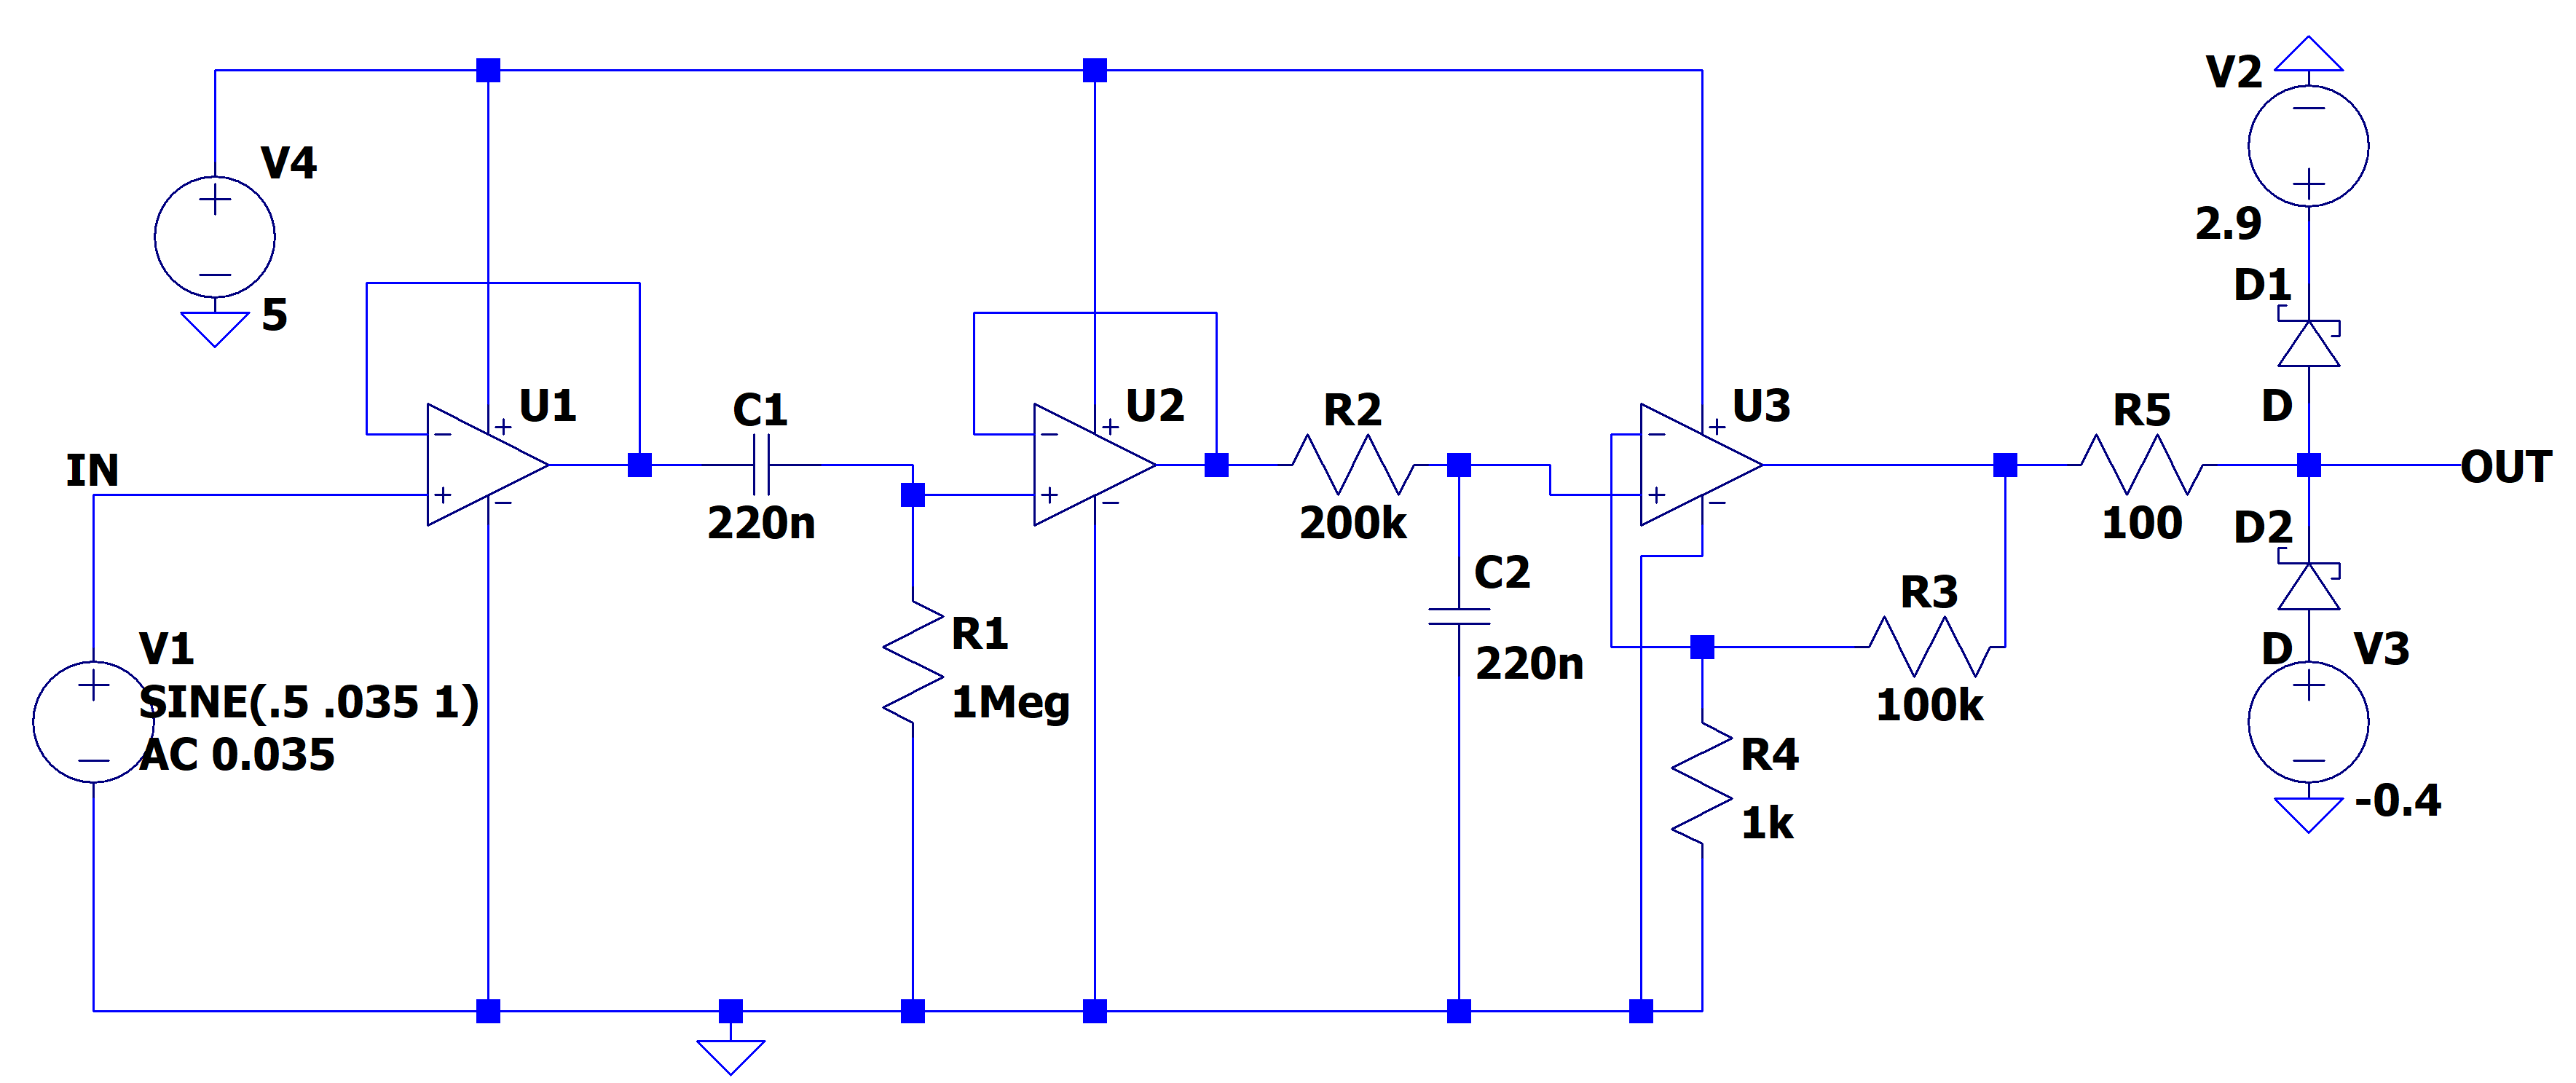
\includegraphics[width=1\textwidth]{LTspiceSchematic.png}
    \caption{LTspice Schematic}
    \label{fig:ltspiceSchematic}
\end{figure}

\section*{Results and Analysis}

\begin{figure}[H]
    \centering
    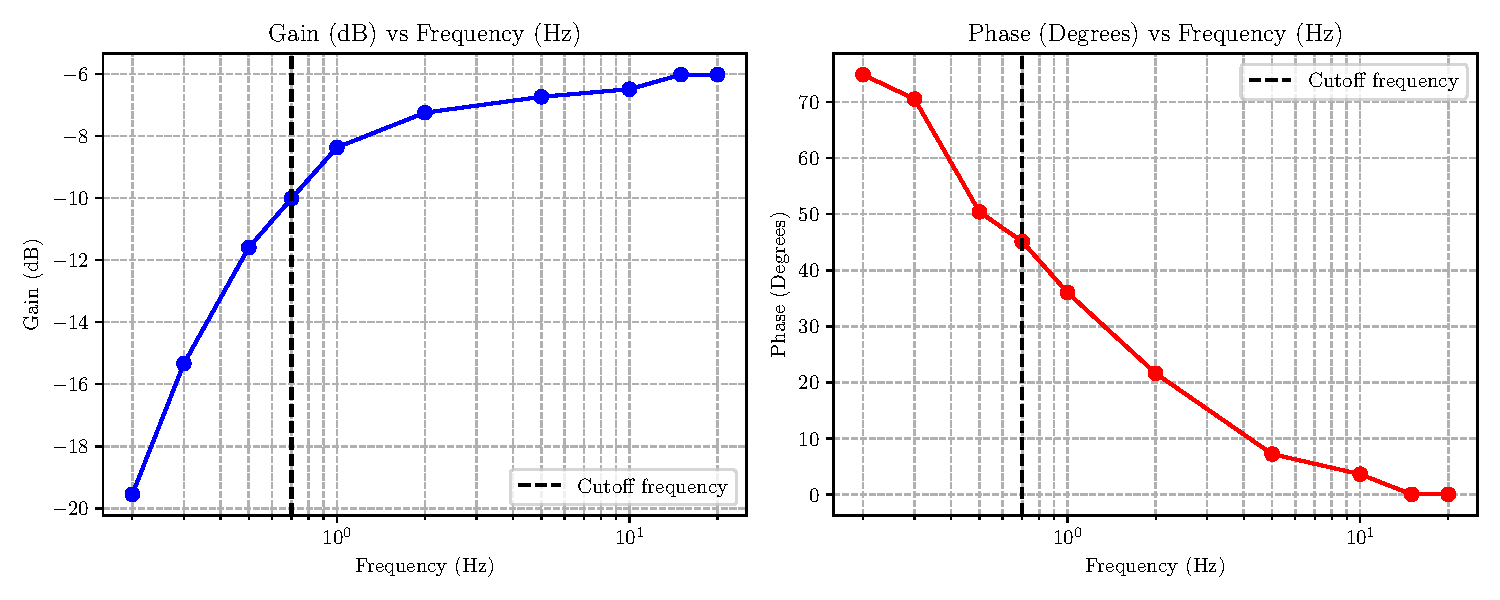
\includegraphics[width=1\textwidth]{high_pass_plot.pdf}
    \caption{High-Pass Filter Bode Plot}
    \label{fig:highPassBode}
\end{figure}

\begin{figure}[H]
    \centering
    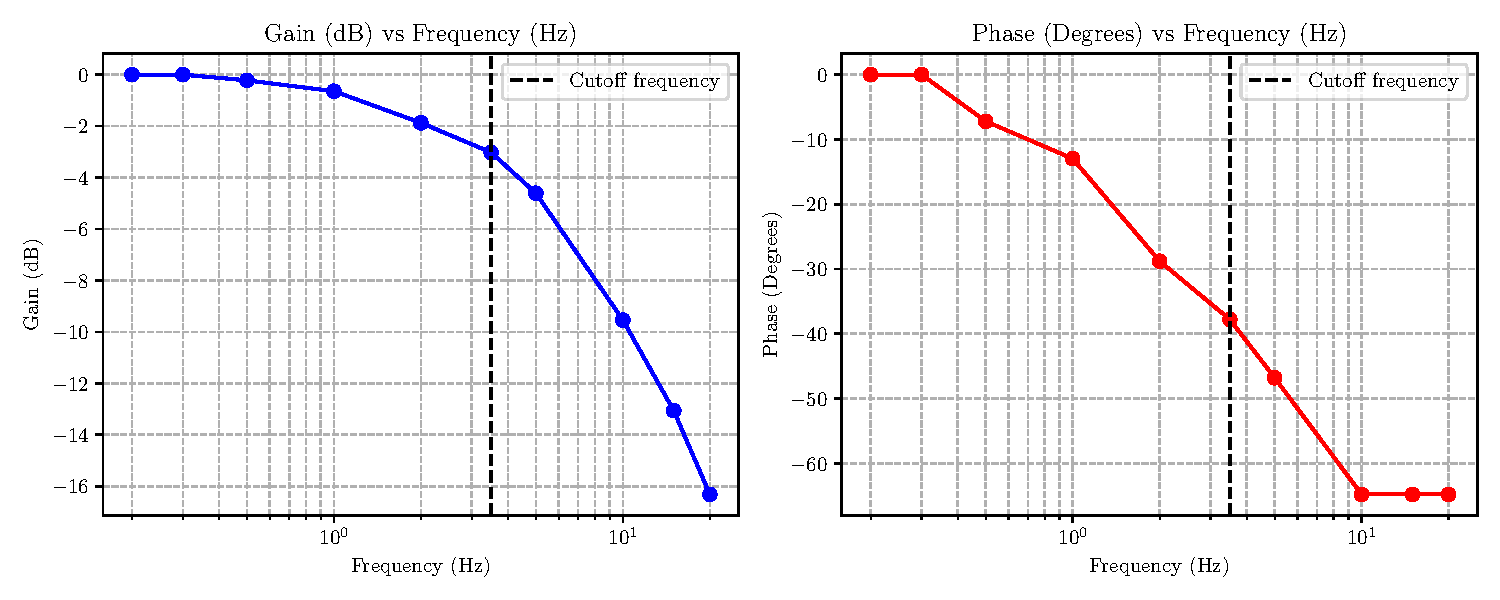
\includegraphics[width=1\textwidth]{low_pass_plot.pdf}
    \caption{Low-Pass Filter Bode Plot}
    \label{fig:lowPassBode}
\end{figure}

\begin{figure}[H]
    \centering
    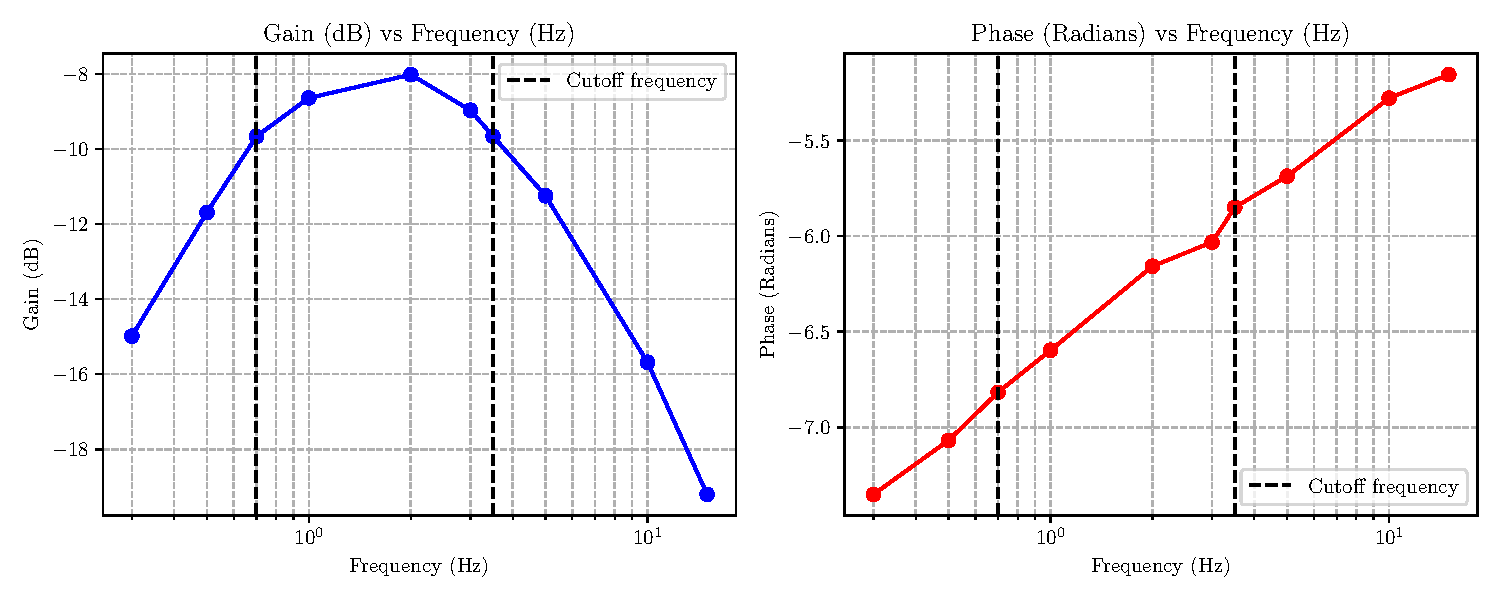
\includegraphics[width=1\textwidth]{band_pass_plot.pdf}
    \caption{Band-Pass Filter Bode Plot}
    \label{fig:bandPassBode}
\end{figure}

\begin{figure}[H]
    \centering
    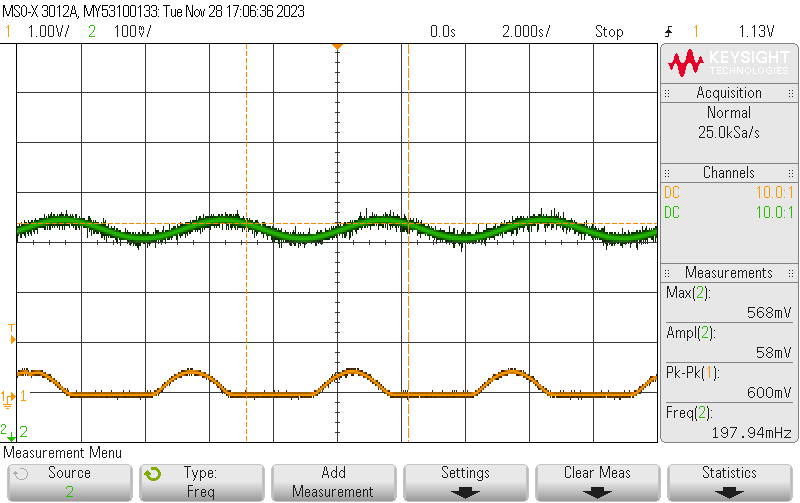
\includegraphics[width=0.75\textwidth]{200mHz.png}
    \caption{Oscilloscope SCHTUFF}
    \label{fig:200mHzCapture}
\end{figure}

\begin{figure}[H]
    \centering
    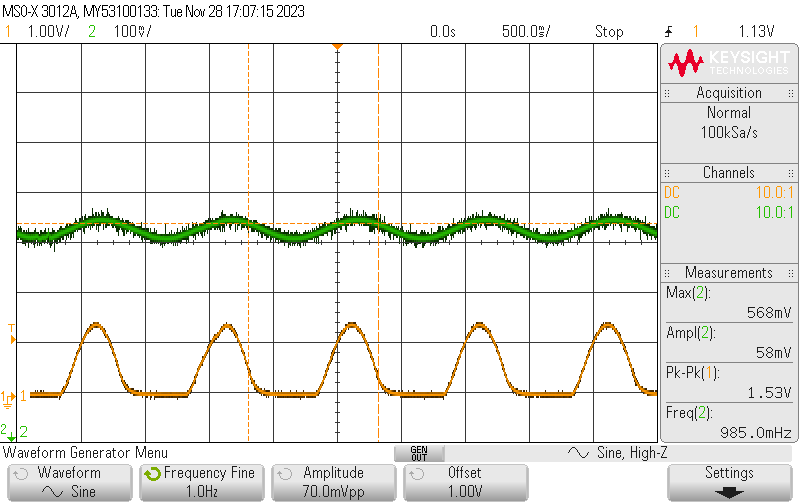
\includegraphics[width=0.75\textwidth]{1Hz.png}
    \caption{Oscilloscope SCHTUFF}
    \label{fig:1HzCapture}
\end{figure}

\begin{figure}[H]
    \centering
    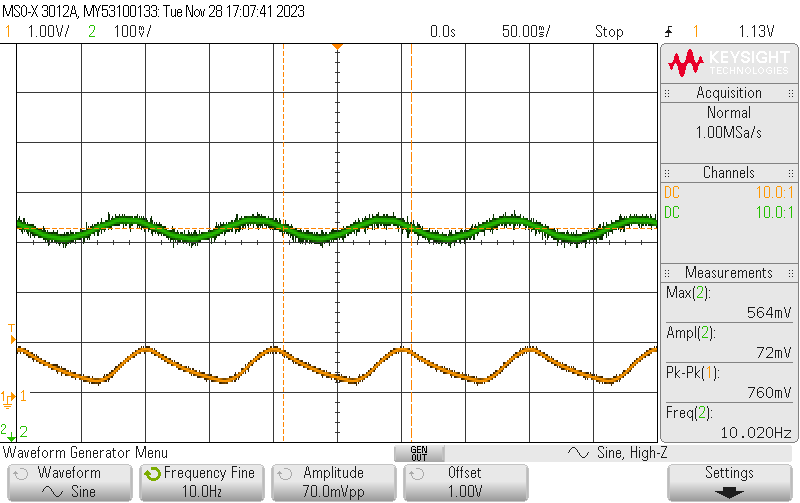
\includegraphics[width=0.75\textwidth]{10Hz.png}
    \caption{Oscilloscope SCHTUFF}
    \label{fig:10HzCapture}
\end{figure}

\section*{Questions}

\textbf{1.} \emph{What is the ERC and DRC for?}

ERC stands for Electrical Rule Check and DRC stands for Design Rule Check. The ERC checks for electrical errors in the schematic, such as unconnected pins. The DRC checks for design errors in the schematic, such as incorrect pin types.

\bigskip

\textbf{2.} \emph{Did your circuit cutoff frequencies match your expected/calculated values? Explain}

\bigskip

\textbf{3.} \emph{Did the gain of the circuit match the expected/calculated values? Explain}

\section*{Conclusion}



\newpage
\begin{figure}[H]
    \centering
    \begin{adjustbox}{center}
        
\includegraphics[width=1.26\textwidth]{signoff.pdf}
    \end{adjustbox}
\end{figure}

\end{document}
